\documentclass{article}

% Official NeurIPS 2026 style (anonymous submission mode, with line numbers for reviewer feedback).
% For a named camera-ready version use \usepackage[final]{neurips_2026}; for a named preprint use [preprint].
\usepackage{neurips_2026}

\usepackage[utf8]{inputenc}
\usepackage[T1]{fontenc}
\usepackage{hyperref}
\usepackage{url}
\usepackage{booktabs}
\usepackage{amsfonts,amsmath,amssymb}
\usepackage{nicefrac}
\usepackage{microtype}
\usepackage{xcolor}
\usepackage{graphicx}
\usepackage{multirow}
\usepackage{enumitem}
\usepackage{tikz}
\usetikzlibrary{arrows.meta,positioning,fit,calc}

\hypersetup{colorlinks=true,linkcolor=blue!50!black,citecolor=blue!50!black,urlcolor=blue!50!black}
\setlist{nosep,leftmargin=1.3em}

% ---- notation and draft markers ----
\newcommand{\phat}{\hat{p}}
\newcommand{\qhat}{\hat{q}}
\newcommand{\blk}[1]{\textsf{#1}}
\newcommand{\tbd}{\textcolor{red!70!black}{TBD}}
\newcommand{\todo}[1]{\textcolor{red!70!black}{[\textbf{TODO:} #1]}}

\title{Will It Follow the Rules? Predicting Instruction Violations\\ from Pre-Generation Internal States}

\author{%
  Anonymous Authors\\
  Course project draft report\\
}

\begin{document}

\maketitle

\begin{abstract}
Language models often break some of the instructions in a prompt when several are given at once, and the failure is
discovered only after a response has been generated and checked. We ask whether a model's violation of each instruction
can be predicted \emph{before} generation, and whether the model's own internal state at the end of the prompt carries
predictive information beyond what a strong reader of the prompt text can extract. We build a controlled
benchmark from ManyIFEval: all 216 tasks are arranged into 72 groups that each share a pool of six sampled, verifiable
rules, and a balanced design over rule subsets ($k=1$ to $5$) and rule orders yields 53,136 prompts. Two
instruction-tuned 8B generators (Llama~3.1 and Qwen3) each produce 20 responses per prompt, every rule is checked with
the official verifiers, and the resulting per-rule and per-prompt violation probabilities serve as targets. We compare
predictors that read the generator's final-prompt-token hidden state or its maximum attention to the target rule's
tokens against frozen text-encoder baselines, under an identical per-rule-type ridge architecture, identical structural
features and identical tuning budgets, in four primary matched comparisons per generator and objective. All modelling
choices are made by grouped cross-validation on 50 training groups, and 22 held-out groups, chosen so that every
compatible pair of rule types appears in at least two of them, remain sealed until the analysis plan is frozen. This draft
specifies the benchmark, the matched-comparison protocol and the evaluation; held-out results are pending.
\end{abstract}

% =====================================================================================================
\section{Introduction}
\label{sec:intro}

People rarely give a language model a single instruction. A typical request names a task and then adds constraints
on length, format, wording and style. Compliance degrades as such constraints accumulate: on ManyIFEval the share of
responses that satisfy every instruction falls steadily as the number of instructions grows from one to ten
\citep{harada2025instructions}, and the same pattern continues at hundreds of instructions \citep{jaroslawicz2025many}.
The failure is also silent. A user learns that a rule was broken only after the response is written and checked, by a
person or a verifier.

If the probability that each rule will be violated could be estimated before generation, a system could restate or
reorder a risky rule, route the prompt to a stronger model, or sample more candidates. At that moment two sources of
information exist: the prompt, which any external model can read, and the generating model's internal state after
reading it. Probing work shows that hidden states predict whether an answer will be correct
\citep{kadavath2022know,azaria2023internal,orgad2025llms}, and recent work finds directions that track whether a single
instruction will be followed \citep{heo2025know}. Attention to the tokens that encode a constraint has been shown to
predict whether factual constraints are satisfied \citep{yuksekgonul2024attention}.

What is much less clear is how much of this signal is specific to the model's internals. Whether a rule is violated
depends strongly on what the rule asks: a requirement of exactly three paragraphs fails far more often than a ban on
commas, and both facts can be read directly from the prompt. A probe on hidden states can therefore perform well
merely because the prompt is encoded in them. The question that matters for practice is the incremental one:
\emph{does the generator's internal state predict its violations better than an equally well-tuned predictor that sees
only the prompt?} Existing studies rarely answer it: labels are usually one sampled response per prompt, so the target
is mostly sampling noise; prompts are observational, so rule identity, count, order and task vary together; and probes
are compared with weak or differently structured baselines, so any gap mixes the value of the representation with
differences in architecture, inputs and tuning.

We design a study that answers the incremental question for prompts with several simultaneous rules:
\begin{itemize}
\item \textbf{A controlled multi-rule benchmark with probabilistic labels} (Section~\ref{sec:data}). From all 216
ManyIFEval tasks we build 72 three-task groups, each with its own pool of six jointly satisfiable rules sampled from the
released code, and a balanced design of nested rule subsets with component-orthogonal-array orderings. This gives
53,136 prompts, 221,616 prompt--rule targets and 2.1 million verified responses from two generators, plus a held-out
expansion covering every rule subset of the test groups.
\item \textbf{Matched comparisons that isolate the representation} (Section~\ref{sec:methods}). Every per-rule predictor uses the same 15 rule-type ridge heads, structural features, exact-rule embedding where
relevant, and penalty grid. Each primary comparison swaps exactly one block, the
representation of the prompt: a frozen text embedding, the generator's hidden state, or its maximum attention to the
target rule. 
\item \textbf{A pre-specified, group-level evaluation} (Section~\ref{sec:experiments}). Selection uses only grouped
cross-validation on 50 training groups. A 22-group test split guarantees that every compatible pair of rule types
co-occurs in at least two held-out pools. Effects are reported as paired differences with group-bootstrap intervals, a
cross-generator control, calibration, and controlled analyses of rule position, count, composition and task.
\end{itemize}
The held-out groups have not been read; this draft specifies the experiments fully and marks test results as
pending.

% =====================================================================================================
\section{Related work}
\label{sec:related}

\paragraph{Following many instructions at once.} IFEval introduced instructions whose compliance can be checked by a
program, such as word counts, required keywords and formatting \citep{zhou2023ifeval}. ManyIFEval combines up to ten of
15 IFEval instruction types in one prompt, shows that compliance declines with the number of instructions, and
estimates performance on unseen combinations from the instruction count \citep{harada2025instructions}. FollowBench
\citep{jiang2024followbench} adds constraints level by level, InFoBench \citep{qin2024infobench} decomposes
requirements into yes/no questions, ComplexBench \citep{wen2024complexbench} composes constraints with logical
structure, IFBench \citep{pyatkin2025ifbench} tests generalisation to unseen verifiable constraints, Multi-IF
\citep{he2024multiif} extends IFEval to multi-turn and multilingual settings, and IFScale \citep{jaroslawicz2025many}
pushes the count to hundreds of keyword instructions. Compliance also depends on where a constraint appears
\citep{zeng2025order,liu2024lost} and on superficial prompt formatting \citep{sclar2024quantifying}. These works
measure compliance after generation. We predict, for one prompt and one rule, the probability of violation before any
token is generated, and our balanced design turns the documented order and composition effects into controlled
factors.

\paragraph{Probing internal states.} Linear and shallow probes are the standard tool for asking what a representation
encodes \citep{alain2016probes,belinkov2022probing}, with the caveat that an expressive probe can learn the task rather
than reveal the representation \citep{hewitt2019control}. Probes detect whether a statement is true \citep{azaria2023internal,burns2023discovering,marks2023geometry,li2023iti,zou2023repe}, whether the
model knows an answer \citep{kadavath2022know}, whether a generation is likely to be hallucinated
\citep{kossen2024sep,orgad2025llms}, and how much a model knows about an entity before generating anything
\citep{gottesman2024estimating}. Closest to us, \citet{heo2025know} find a direction in input representations that
predicts whether a response will follow a single IFEval instruction and that generalises across tasks but not across
instruction types, and \citet{stolfo2025steering} steer format and length compliance with activation differences.
\citet{ashok2025predict} train probes on input-token states to forecast behaviours of the whole output, and
\citet{rocchetti2026follow} report that probe signal for constraint satisfaction is weak before generation and grows
during it. We differ in four respects: prompts carry several rules, each a separate target; labels are probabilities
from 20 samples per prompt; the comparators are text-only predictors with the same head, features and supervision; and
a cross-generator control asks whether the signal is specific to the model that generates the response. The last two
address the probing caveat: a probe that wins only by encoding the prompt should not beat a matched text encoder or the
other generator's states.

\paragraph{Attention as a predictive signal.} SAT Probe treats a factual query as a set of constraints and shows that
the maximum attention from the final token to each constraint's tokens predicts whether the model will satisfy it
\citep{yuksekgonul2024attention}. Lookback Lens detects contextual hallucinations from the ratio of attention on the
context to attention on generated tokens \citep{chuang2024lookback}, and PASTA improves instruction following by
up-weighting attention to user-marked spans \citep{zhang2024pasta}. We carry the SAT Probe construction over to instruction-rule spans and compare it with hidden states and text
embeddings under matched conditions. We take the span maximum rather than the sum because much attention mass sits on
``sink'' tokens \citep{xiao2024sinks}, and treat attention as a predictive feature, not an explanation
\citep{jain2019attention,wiegreffe2019attention}.

\paragraph{Uncertainty, self-evaluation and routing.} Calibration \citep{guo2017calibration} has been studied for language models through verbalised confidence \citep{lin2022teaching,tian2023just,xiong2024express},
self-evaluation \citep{kadavath2022know}, and sampling-based semantic uncertainty
\citep{kuhn2023semantic,farquhar2024detecting}, which semantic entropy probes approximate from a single forward pass
\citep{kossen2024sep}. For instruction following, \citet{heo2025uncertainty} find that internal-state estimators beat
verbalised and logit-based ones but approach chance in their hardest controlled setting. Routers pick a model before generation \citep{ding2024hybrid,ong2025routellm}. Most of these estimators score an
existing response or general answer quality; ours run before generation and target each explicit constraint, with
probabilistic labels that make calibration a natural secondary metric.

% =====================================================================================================
\section{Problem formulation}
\label{sec:problem}

A prompt $x$ consists of a task description followed by an ordered list of $k\le 5$ rules $(r_1,\dots,r_k)$. A
generator $G$ samples a response $y\sim G(\cdot\mid x)$, and a deterministic verifier returns $c_r(y)\in\{0,1\}$ for
each rule, with $1$ meaning violated. The quantities of interest are properties of the response distribution:
\begin{equation}
p_r(x)=\Pr_{y\sim G(\cdot\mid x)}\!\left[c_r(y)=1\right],\qquad q(x)=\frac{1}{k}\sum_{j=1}^{k}p_{r_j}(x).
\label{eq:targets}
\end{equation}
We estimate them from $n=20$ independent samples: $\phat_r(x)=v_r(x)/n$, where $v_r$ counts violating responses, and
$\qhat(x)$ is the mean of $\phat$ over the prompt's rules. $q$ is the expected \emph{fraction} of rules violated, not
the probability that at least one is. \textbf{Objective~1} is to predict $p_r(x)$ for every prompt--rule pair;
\textbf{Objective~2} is to predict $q(x)$ for every prompt. Predictors may use only the prompt text, its
known structure and the generator's activations on the prompt; responses serve only as labels. The two generators are
separate experiments.

% =====================================================================================================
\section{A controlled multi-rule benchmark}
\label{sec:data}

\begin{figure}[t]
\centering
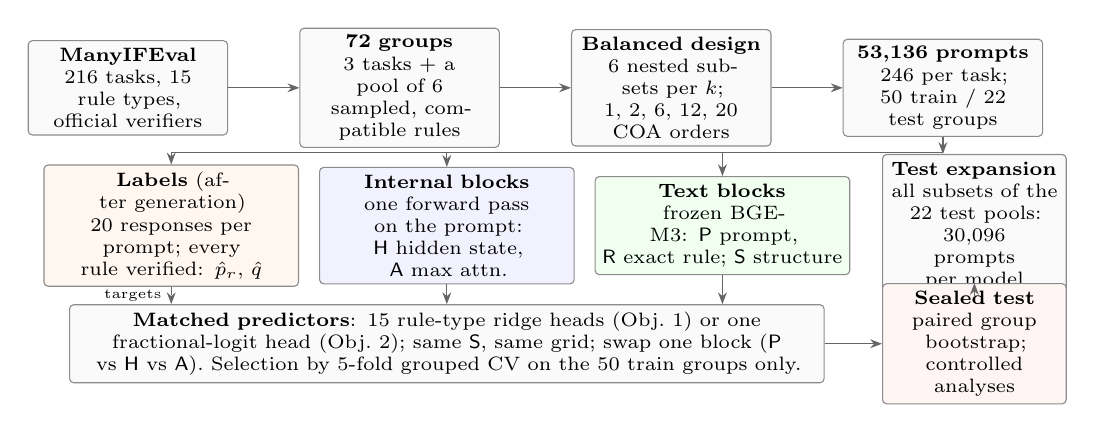
\begin{tikzpicture}[font=\scriptsize,
  box/.style={draw=black!45, rounded corners=1.5pt, align=center, inner sep=2.6pt, text width=#1, fill=black!2},
  box/.default=2.35cm, arr/.style={-{Stealth[length=1.5mm]}, draw=black!60, line width=0.45pt}]
\node[box] (src) at (0,0) {\textbf{ManyIFEval}\\216 tasks, 15 rule types,\\official verifiers};
\node[box] (grp) at (3.45,0) {\textbf{72 groups}\\3 tasks + a pool of 6\\sampled, compatible rules};
\node[box] (des) at (6.9,0) {\textbf{Balanced design}\\6 nested subsets per $k$;\\1, 2, 6, 12, 20 COA orders};
\node[box] (pr) at (10.35,0) {\textbf{53,136 prompts}\\246 per task;\\50 train / 22 test groups};
\draw[arr] (src) -- (grp); \draw[arr] (grp) -- (des); \draw[arr] (des) -- (pr);
\node[box=3.05cm, fill=orange!6] (lab) at (0.55,-1.75) {\textbf{Labels} (after generation)\\20 responses per prompt; every\\rule verified: $\phat_r$, $\qhat$};
\node[box=3.05cm, fill=blue!5] (int) at (4.05,-1.75) {\textbf{Internal blocks}\\one forward pass on the prompt:\\\blk{H} hidden state, \blk{A} max attn.};
\node[box=3.05cm, fill=green!6] (txt) at (7.55,-1.75) {\textbf{Text blocks}\\frozen BGE-M3: \blk{P} prompt,\\\blk{R} exact rule; \blk{S} structure};
\node[box=2.15cm] (exp) at (10.75,-1.75) {\textbf{Test expansion}\\all subsets of the\\22 test pools: 30,096\\prompts per model};
\coordinate (bus) at (10.35,-0.82);
\draw[draw=black!60, line width=0.45pt] (pr.south) -- (bus);
\draw[arr] (bus) -| (lab.north); \draw[arr] (bus) -| (int.north); \draw[arr] (bus) -| (txt.north); \draw[arr] (bus) -- ($(exp.north)+(-0.4,0)$);
\node[box=9.4cm] (hd) at (4.05,-3.25) {\textbf{Matched predictors}: 15 rule-type ridge heads (Obj.~1) or one fractional-logit head (Obj.~2);
same \blk{S}, same grid; swap one block (\blk{P} vs \blk{H} vs \blk{A}). Selection by 5-fold grouped CV on the 50 train groups only.};
\draw[arr] (int.south) -- (int.south |- hd.north); \draw[arr] (txt.south) -- (txt.south |- hd.north);
\draw[arr, dashed] (lab.south) -- (lab.south |- hd.north) node[midway, left, font=\tiny] {targets};
\node[box=2.15cm, fill=red!4] (ev) at (10.75,-3.25) {\textbf{Sealed test}\\paired group bootstrap;\\controlled analyses};
\draw[arr] (hd.east) -- (ev.west); \draw[arr] (exp.south) -- (ev.north);
\end{tikzpicture}
\caption{Overview. Each generator supplies labels (from sampled responses) and internal feature blocks (from one
forward pass on the prompt alone). Predictors that differ only in the prompt-representation block are compared on
held-out groups.}
\label{fig:overview}
\end{figure}

\paragraph{Source.} We use the released ManyIFEval repository \citep{harada2025instructions} at a pinned commit: its 216
task descriptions, its 15 instruction types (Appendix~\ref{app:types}) and the official verifier of each type, which
come from IFEval \citep{zhou2023ifeval}. Our serialiser reproduces all 2,160 released prompts byte for byte.

\paragraph{Groups and rule pools.} All 216 tasks are used. Each task receives one of six family labels
(informational, creative, persuasive, practical, analytical, transformation) from a written rubric; the labels are our
proposal, not part of ManyIFEval. A scripted version of the rubric, frozen before comparison, agrees with the hand labels
on 88.0\% of tasks (Cohen's $\kappa=0.85$; \citealp{landis1977kappa}). Tasks are formed into 72 groups of three from
different families. Each group receives its own pool of six rules with six distinct types. Types that ManyIFEval never combines (\{keyword existence, frequency\}, the three letter-case types, \{word,
sentence, paragraph count\}) are incompatible. Parameters are drawn by
calling each released instruction class's default generator, so the released code alone defines their distribution. A
draw is rejected only if it is provably unsatisfiable or contradicts another rule in the pool, and a pool is accepted
only when a constructed witness response passes all six official verifiers for each of the group's three tasks. As in the
released prompts, there is no filter on how natural a rule is for a task. The 432 rule instances are fixed within their
group and sampled independently across groups.

\paragraph{Rule subsets and orders.} Within a group the six rules are placed in one random cyclic order. The six
rotations of that order, cut to five rules, form six \emph{chains}, and the first $k$ rules of a chain form a subset,
for $k=1,\dots,5$. Every $k$ therefore has six subsets, each rule appears in exactly $k$ of them, and subsets are nested
along a chain, so appending one rule is a controlled change. Each subset is presented in 1, 2, 6, 12 or 20 orders for
$k=1,\dots,5$, taken from an index-one, strength-two component orthogonal array (COA; \citealp{yang2021coa}): for $k\ge
2$ every rule occupies every position equally often and every ordered pair of rules occupies every pair of positions
exactly once (constructions in Appendix~\ref{app:design}). The three tasks of a group share the same 246 ordered rule lists, so task effects are controlled too. A prompt is the
task text, ManyIFEval's fixed header and one bullet per rule.

\paragraph{Responses and labels.} The generators are \texttt{Llama-3.1-8B-Instruct} \citep{grattafiori2024llama3} and
\texttt{Qwen3-8B} \citep{yang2025qwen3} with thinking disabled, at pinned revisions and in bfloat16 without
quantisation. Each prompt is one user turn rendered with the model's chat template. We draw 20 responses per prompt with
each model card's default decoding (Llama: temperature 0.6, top-$p$ 0.9; Qwen: temperature 0.7, top-$p$ 0.8, top-$k$
20) and at most 2,048 new tokens, using vLLM \citep{kwon2023vllm} on NVIDIA B200 GPUs. No prompt is truncated. Every rule is checked on every response with its official verifier (empty responses fail), with the verifiers'
language detection and sentence splitter seeded or pinned. Truncated and looping responses are kept.

\paragraph{Split.} Groups are the unit of independence, because the prompts of a group share tasks, rules and orders.
We hold out 22 of the 72 groups (Table~\ref{tab:counts}). The split was chosen from pool metadata alone by a seeded search over
20,000 random assignments refined by swaps (Appendix~\ref{app:split}). It requires that every compatible pair of rule types (98 pairs) co-occur in the pool of at least two test groups
and at least one training group, that every type appear in at least one test and five training groups, and that
clusters of near-duplicate tasks stay on one side; it then minimises the family and type imbalance between test and full data. One pair occurs in only two pools overall and is test-only. In
the resulting split every pair co-occurs in 2 to 8 test groups and
each type appears in 6 to 12 test and at least 10 training groups. Test rules share types (and, for parameter-free types,
wording) with training rules, so the test set measures generalisation to unseen tasks and rule combinations, not to
unseen rule types.

\begin{table}[t]
\centering\small
\caption{Dataset size per generator under the adopted split. Prompt--rule rows are the units of Objective~1 and prompts
the units of Objective~2. The expansion adds every remaining rule subset at $k=2,3,4$ for the 22 test groups.}
\label{tab:counts}
\setlength{\tabcolsep}{5pt}
\begin{tabular}{lrrrrr}
\toprule
 & Per task & Train (50 groups) & Test (22 groups) & Test expansion & All \\
\midrule
Tasks & 1 & 150 & 66 & (same 66) & 216 \\
Prompts & 246 & 36,900 & 16,236 & +13,860 & 66,996 \\
Prompt--rule rows & 1,026 & 153,900 & 67,716 & +47,520 & 269,136 \\
Responses & 4,920 & 738,000 & 324,720 & +277,200 & 1,339,920 \\
\bottomrule
\end{tabular}
\end{table}

\paragraph{Held-out expansion for controlled analyses.} The design has only six of the $\binom{6}{k}$ subsets per $k$, so some matched comparisons
(e.g.\ replacing one companion rule) have few pairs. For the 22 test groups only, we add every other subset at
$k=2,3,4$ with the same COA template: 456 rule lists per task, 30,096 test prompts per generator. Original prompts keep
their responses; new responses use the same models, decoding and engine. This generation is in progress, and no test
response is verified before the analysis plan is frozen.

\paragraph{Pre-generation features.} For each prompt and generator we run one forward pass on the rendered prompt and
read everything at the \emph{final prompt token}, the position from which the first response token is sampled. We store
the 4,096-dimensional hidden state after every layer and, for every layer $l$ and head $h$, the maximum attention weight
from that token to the tokens of each rule's exact span,
\begin{equation}
A_{l,h}(r)=\max_{t\in\mathrm{span}(r)}\alpha^{(l,h)}_{T,t},
\label{eq:maxattn}
\end{equation}
where $T$ is the final prompt token. This gives $32\times32=1{,}024$ values per rule for Llama and $36\times32=1{,}152$
for Qwen. Features are computed with Hugging Face Transformers (eager, bfloat16) on Apple silicon, not on the generation
backend; a 100-prompt check found identical tokens and hidden-state cosine $\ge0.998$ across backends.

% =====================================================================================================
\section{Matched predictors}
\label{sec:methods}

\subsection{Feature blocks and predictors}

Every predictor is a regularised generalised linear model on a concatenation of feature blocks (dimensions for
Objective~1):
\begin{itemize}
\item \blk{S}, \textbf{structure} (20 columns): $k$, the target rule's position, indicators for the 15 types of the
companion rules, the rendered prompt length, the target span length and the distance from the span to the final token,
all counted in the target generator's tokens. Parsed rule parameters, task and group identifiers are never inputs.
\item \blk{P}, \textbf{prompt embedding} (1,024): the frozen, pinned BGE-M3 dense embedding \citep{chen2024bge} of the
full prompt.
\item \blk{R}, \textbf{exact-rule embedding} (1,024): the same encoder applied to the target rule's wording alone.
\item \blk{H}, \textbf{hidden state} (4,096): the generator's final-token hidden state at one selected layer.
\item \blk{A}, \textbf{rule attention} (1,024 or 1,152): Eq.~\eqref{eq:maxattn} for the target rule, all layers and
heads.
\end{itemize}
\blk{P}, \blk{H} and \blk{A} are alternative representations of the prompt, from an independent text encoder or from
the generator itself; \blk{R} identifies the exact target rule. The predictors are combinations of these blocks
(Table~\ref{tab:predictors}): B1 $=$ \blk{S}+\blk{P} and B2 $=$ \blk{S}+\blk{P}+\blk{R} are text-only baselines; H1 $=$
\blk{S}+\blk{H} and H2 $=$ \blk{S}+\blk{H}+\blk{R} are hidden-state probes; the rule-conditioned attention probe (RCAP)
is \blk{S}+\blk{A}+\blk{R}; and B1+H1, B2+H1 and B2+A1 add an internal block to a baseline.

\begin{table}[t]
\centering\small
\caption{Predictors, their blocks, and the comparisons. In every primary comparison the two sides share \blk{S}, the
head architecture and the tuning grid, and differ only in the prompt-representation block. ``Right minus left'' in
loss is positive when the left predictor is better.}
\label{tab:predictors}
\setlength{\tabcolsep}{4pt}
\begin{tabular}{clllp{3.6cm}}
\toprule
\# & Left & Right & Swap & Question \\
\midrule
1 & H1 (\blk{S}+\blk{H}) & B1 (\blk{S}+\blk{P}) & \blk{H} / \blk{P} & hidden state vs prompt text \\
2 & H2 (\blk{S}+\blk{H}+\blk{R}) & B2 (\blk{S}+\blk{P}+\blk{R}) & \blk{H} / \blk{P} & same, given the exact rule \\
3 & RCAP (\blk{S}+\blk{A}+\blk{R}) & B2 (\blk{S}+\blk{P}+\blk{R}) & \blk{A} / \blk{P} & rule attention vs prompt text \\
7 & H2 (\blk{S}+\blk{H}+\blk{R}) & RCAP (\blk{S}+\blk{A}+\blk{R}) & \blk{H} / \blk{A} & hidden state vs rule attention \\
\midrule
4 & B1+H1 & B1 (frozen) & $+\blk{H}$ & increment of \blk{H} over B1 \\
5 & B2+H1 & B2 (frozen) & $+\blk{H}$ & increment of \blk{H} over B2 \\
6 & B2+A1 & B2 (frozen) & $+\blk{A}$ & increment of \blk{A} over B2 \\
\midrule
\multicolumn{5}{p{12.6cm}}{References: structure only (\blk{S}); other generator's H1 (\blk{S} + the \emph{other}
model's \blk{H}); for Obj.~2, Obj.~1 predictions averaged per prompt.}\\
\bottomrule
\end{tabular}
\end{table}

\subsection{Heads and losses}

\textbf{Objective~1.} Every predictor has 15 heads, one per rule type; a prompt--rule row is routed to the head of its
rule's type. Parameter variants of a type share weights, and no exact rule has its own head. Head $\tau$ predicts
$\hat p=\sigma(\mathbf{w}^\top\mathbf{z}+b)$ from the standardised block concatenation $\mathbf{z}$ and is fitted on
violation and compliance counts by penalised binomial likelihood,
\begin{equation}
\min_{\mathbf{w},b}\;-\sum_{i\in\tau}\Big[v_i\log\hat p_i+(n-v_i)\log(1-\hat p_i)\Big]
+\lambda_S\lVert\mathbf{w}_S\rVert_2^2+\lambda_X\lVert\mathbf{w}_X\rVert_2^2+\lambda_R\lVert\mathbf{w}_R\rVert_2^2,
\label{eq:obj1}
\end{equation}
where $X\in\{P,H,A\}$ is the predictor's prompt-representation block. The summed loss gives every head the same prior
strength whatever its size; standardisation uses each head's fitting rows only.

\textbf{Objective~2.} Every predictor has one shared head per generator. Per-rule blocks are averaged over the prompt's
rules ($\bar{\blk{R}}$, $\bar{\blk{A}}$), so all rules share one set of weights, and \blk{S} becomes 92 columns: $k$,
prompt length, and for each of five ordered slots the rule type, span length, distance to the final token and a
presence mask. The head is a ridge-penalised fractional logit \citep{papke1996fractional}: the loss in
Eq.~\eqref{eq:obj1} with $\qhat$ as a soft label and every prompt weighted equally, rather than counting its $20k$
checks as separate examples. A sensitivity analysis keeps them in ordered slots.

\subsection{Tuning, with identical budgets}

\textbf{Penalty slots.} The structure penalty $\lambda_S$ is fixed, weak and identical in every predictor (10 for
Objective~1, 1 for Objective~2, on the summed-loss scale). The prompt-representation penalty $\lambda_X$ and the
rule-embedding penalty $\lambda_R$ are each tuned over the same six values, spaced by factors of 10 ($10^2$ to $10^7$
for Objective~1, $10^0$ to $10^5$ for Objective~2). If any predictor selects an edge value, that slot's grid is extended by one step in that
direction, once, for every predictor that uses it. Ties in pooled loss (at a recorded precision) go to the setting with
the largest total log-penalty, then to the larger $\lambda_X$, so selection is deterministic.

\textbf{Incremental comparisons.} For comparisons 4--6 the baseline is frozen at its own selection, and only the added
block's penalty is tuned, over the same six values plus ``off''. If ``off'' is chosen, the gain is zero by construction,
which we do not read as evidence that the block is uninformative.

\textbf{Hidden layer.} Five candidate layers per generator, at 25\%, 37.5\% (38.9\% for Qwen), 50\%, 75\% and 100\% of
depth, are compared with H1 for each objective, and the selected layer is reused by every hidden-state predictor of that
generator and objective. Hidden-state predictors thus receive a five-way layer search that text and attention
predictors do not, which we disclose next to every result. \blk{A} always uses all layers and heads.

\textbf{Sparse heads.} A rule-type head whose fitting rows contain fewer than 50 violated or 50 compliant completions,
or violations in fewer than 5 groups, is replaced by the intercept-only estimate $(v+0.5)/(n+1)$. The decision depends
only on labels, so a fallback type contributes identical predictions to both sides of every comparison.

\textbf{Selection and refit.} The 50 training groups are split into five folds of ten groups (GroupKFold). Settings are
selected by pooled held-out loss: mean log loss per completion for Objective~1 and squared error of $\hat q$ for
Objective~2. Selected settings are refitted on all 50 training groups, and these refitted models are the ones applied
once to the test groups. The recipe, grids, thresholds and tie rule were hashed before any selection ran.

% =====================================================================================================
\section{Experiments}
\label{sec:experiments}

\subsection{Protocol}

\paragraph{Test-set discipline.} No feature, label or prediction of a test group has been computed or read; the loaders
refuse test rows until unblinding is recorded, and an automated test guards this. The plan below will be frozen and
hashed with the fitted models before unblinding. Selection by cross-validation makes the training losses of selected settings optimistic
\citep{cawley2010overfitting}, so we use them only to choose settings and report them only as diagnostics
(Appendix~\ref{app:cv}).

\paragraph{Primary metrics.} For Objective~1 the primary effect is the change in pooled mean log loss per completion,
right minus left, so that a positive value favours the left predictor in every row of Table~\ref{tab:predictors}. For
Objective~2 it is the change in root mean squared error of $\hat q$ with every prompt weighted equally.

\paragraph{Uncertainty.} The group is the unit of resampling. A paired group bootstrap \citep{efron1979bootstrap} draws whole test groups with replacement, using the same
10,000 draws for every predictor, and gives pointwise 95\% percentile intervals; a leave-one-group-out jackknife with a
$t_{21}$ interval is a small-sample check. Intervals are unadjusted, the four primary comparisons are pre-specified,
and an interval spanning zero is not read as equal performance.

\paragraph{Secondary metrics.} For Objective~1: the change in per-completion ROC AUC (half credit for ties), the number of
evaluable rule types on which the left predictor has lower log loss, and test groups favouring each side. For Objective~2: the
change in mean absolute error, and RMSE and MAE by $k$. For both: expected calibration error and reliability diagrams
\citep{guo2017calibration}, with bins fixed from training predictions.

\paragraph{Controlled analyses.} The balanced design, completed by the test expansion, supports matched pairs in which
one property of the prompt changes and everything else is fixed: (A)~\emph{position}, the target rule moves within the
same ordered set; (B)~\emph{count}, one rule is appended ($k\to k+1$); (C)~\emph{composition}, one companion rule is
replaced at the same $k$ and target position; and (D)~\emph{task}, the same ordered rules are attached to another task
of the group. For each pair we compare the predicted change in risk with the observed change, scoring the mean absolute
error of the change and, on pairs whose observed change is reliably non-zero, the accuracy of its sign. This asks
whether a predictor tracks how risk changes, not only its level.

\paragraph{Sensitivity analyses.} Primary metrics are recomputed without the ``all uppercase'' rule (its verifier's
language detection can reject correct uppercase English), without truncated responses, and without looping prompts.

\paragraph{How the outcomes will be read.} Comparisons 2 and 3 are the central test: if hidden state or rule attention beats B2, which
already sees the prompt, the exact rule and the structure, the internal state exposes information to a linear head that
a frozen encoder of the same prompt does not. Comparison 7 asks which internal signal is more useful. The
other-generator reference separates self-specific signal from a better encoding of the prompt: if Qwen's states predict
Llama's labels as well as Llama's own, the advantage is representational, not self-knowledge.

\paragraph{Training-side status.}

Selection and refitting are complete (Appendix~\ref{app:cv}); CV selected layer 12
(37.5\% depth) for Llama and layers 18 and 27 (50\%, 75\%) for Qwen in Objectives~1 and~2.

\subsection{Results}
\label{sec:results}

\begin{table}[t]
\centering\small
\caption{Primary comparisons on the 22 held-out groups (\emph{pending unblinding}). $\Delta$ is right minus left, so
positive values favour the left predictor. Intervals: paired group bootstrap, 95\%, pointwise. ``Types'': evaluable rule
types on which the left predictor has lower log loss.}
\label{tab:main}
\setlength{\tabcolsep}{3.3pt}
\begin{tabular}{llcccccc}
\toprule
 & & \multicolumn{3}{c}{Objective 1 (per rule)} & \multicolumn{2}{c}{Objective 2 (per prompt)} \\
\cmidrule(lr){3-5}\cmidrule(lr){6-7}
Gen. & Comparison (left vs right) & $\Delta$ log loss [95\% CI] & $\Delta$ AUC & Types & $\Delta$ RMSE [95\% CI] & $\Delta$ MAE \\
\midrule
\multirow{4}{*}{Llama} & 1: H1 vs B1 & \tbd{} [\tbd, \tbd] & \tbd & \tbd/15 & \tbd{} [\tbd, \tbd] & \tbd \\
 & 2: H2 vs B2 & \tbd{} [\tbd, \tbd] & \tbd & \tbd/15 & \tbd{} [\tbd, \tbd] & \tbd \\
 & 3: RCAP vs B2 & \tbd{} [\tbd, \tbd] & \tbd & \tbd/15 & \tbd{} [\tbd, \tbd] & \tbd \\
 & 7: H2 vs RCAP & \tbd{} [\tbd, \tbd] & \tbd & \tbd/15 & \tbd{} [\tbd, \tbd] & \tbd \\
\midrule
\multirow{4}{*}{Qwen} & 1: H1 vs B1 & \tbd{} [\tbd, \tbd] & \tbd & \tbd/15 & \tbd{} [\tbd, \tbd] & \tbd \\
 & 2: H2 vs B2 & \tbd{} [\tbd, \tbd] & \tbd & \tbd/15 & \tbd{} [\tbd, \tbd] & \tbd \\
 & 3: RCAP vs B2 & \tbd{} [\tbd, \tbd] & \tbd & \tbd/15 & \tbd{} [\tbd, \tbd] & \tbd \\
 & 7: H2 vs RCAP & \tbd{} [\tbd, \tbd] & \tbd & \tbd/15 & \tbd{} [\tbd, \tbd] & \tbd \\
\bottomrule
\end{tabular}
\end{table}

\todo{After unblinding: fill Table~\ref{tab:main} from saved tables; add the secondary table (comparisons 4--6 and
references), reliability diagrams, per-type results and a predicted-vs-observed-change figure for analyses A--D; then
analyse internal vs text (1--3), hidden vs attention (7), increments (4--6), own vs other generator, where gains
concentrate, calibration, and sensitivity.}

% =====================================================================================================
\section{Discussion and limitations}
\label{sec:discussion}

\paragraph{What the design can and cannot show.} The matched comparisons answer a predictive question: given the same
head, structure, rule identity and tuning budget, is one representation of the prompt more useful than another for
forecasting a specific model's violations? A win for hidden state or attention would show that this information is more accessible to a regularised linear
readout in the generator's activations than in a strong text embedding, not that the model ``knows'' it will fail, uses
this information, or that attention causes violations \citep{jain2019attention,wiegreffe2019attention}. Causal tests, such as steering along probe directions \citep{stolfo2025steering} or re-weighting attention to a
rule \citep{zhang2024pasta}, are the natural next step. Conversely, a loss would show only that the information is not
more linearly available than in the text embedding at the depths searched, not that it is absent.

\paragraph{Limitations.} \emph{Baseline strength.} Both text baselines use a frozen encoder. A fine-tuned encoder (used earlier in the project) was retired for compute, and a stronger prompt
reader, such as a fine-tuned LM or the generator asked to predict its own compliance, could narrow any gap. No
predictor is told a rule's parsed parameters directly. \emph{Asymmetric
search.} Hidden-state predictors receive a five-layer search that the others do not. \emph{Labels.} With 20 samples,
$\phat$ has a standard error of up to 0.11. Verifiers are imperfect; sensitivity analyses cover the known cases. \emph{Backends.} Features come from a different backend
than generation; they approximate the generating states closely but not exactly. \emph{Power and coverage.} Inference
rests on 22 independent test groups. One rule-type pair (uppercase-word count with word count) never co-occurs in
training. \emph{Earlier use of test groups.} Sixteen of the 22 test groups were training groups under an earlier split
and were used in earlier cross-validation and selection, including the choice of default grid values. The final models
are refitted without them, but this prior exposure is a mild form of selection on the test groups.
\emph{Design.} COA orders do not cover all $k!$ orders for $k\ge4$; task-family labels are ours.
\emph{Scope.} Two open 8B models, English prompts, 15 programmatically verifiable rule types, at most five rules, default
decoding and non-thinking mode.

\paragraph{Future work.} Transferring a predictor across generators; locating the layers and heads that carry the attention
signal; and using per-rule risk online (restating risky rules, choosing how many candidates to sample) and measuring
the compliance gain. Larger models, reasoning modes and longer rule lists would test whether findings scale.

% =====================================================================================================
\section{Conclusion}
\label{sec:conclusion}

We test whether a model's internal state, read once at the end of the prompt, predicts which of several instructions
it will violate better than the prompt does. We built a balanced multi-rule benchmark with sampled violation
probabilities for two generators and predictors whose comparisons differ in exactly one block. Training-side selection
is complete and the held-out groups remain sealed. \todo{Summarise the confirmatory findings for comparisons
1--3 and 7, the other-generator control and the controlled analyses, and state the practical implication for
pre-generation risk estimation.}

\bibliographystyle{plainnat}
\bibliography{refs}

% =====================================================================================================
\clearpage
\appendix

\section{Rule types and an example prompt}
\label{app:types}

\begin{table}[h]
\centering\footnotesize
\caption{The 15 rule types, the parameters drawn by the released code's default generators (``rel.'' is ``less than''
or ``at least'', each with probability one half), and the number of training and test groups whose six-rule pool
contains the type under the adopted split.}
\label{tab:types}
\setlength{\tabcolsep}{3pt}\scriptsize
% generated by report/neurips_draft/make_assets.py -- do not edit
\begin{tabular}{lllcc}
\toprule
Rule type & IFEval identifier & Sampled parameters & Train groups & Test groups \\
\midrule
Include keywords & \texttt{\scriptsize keywords:existence} & 2 keywords & 15 & 7 \\
Keyword count & \texttt{\scriptsize keywords:frequency} & 1 keyword, $N\in[1,3]$, rel. & 18 & 8 \\
Forbidden words & \texttt{\scriptsize keywords:forbidden\_words} & 2 keywords & 29 & 11 \\
Letter count & \texttt{\scriptsize keywords:letter\_frequency} & letter, $N\in[1,10]$, rel. & 29 & 12 \\
Word count & \texttt{\scriptsize length\_constraints:number\_words} & $N\in[100,500]$, rel. & 14 & 6 \\
Sentence count & \texttt{\scriptsize length\_constraints:number\_sentences} & $N\in[1,20]$, rel. & 11 & 7 \\
Paragraph count & \texttt{\scriptsize length\_constraints:number\_paragraphs} & $N\in[1,5]$ & 17 & 8 \\
Placeholders & \texttt{\scriptsize detectable\_content:number\_placeholders} & $N\in[1,4]$ & 27 & 10 \\
Bullet points & \texttt{\scriptsize detectable\_format:number\_bullet\_lists} & $N\in[1,5]$ & 25 & 11 \\
Title & \texttt{\scriptsize detectable\_format:title} & none & 26 & 11 \\
All uppercase & \texttt{\scriptsize change\_case:english\_capital} & none & 18 & 8 \\
All lowercase & \texttt{\scriptsize change\_case:english\_lowercase} & none & 10 & 6 \\
Uppercase-word count & \texttt{\scriptsize change\_case:capital\_word\_frequency} & $N\in[1,20]$, rel. & 12 & 6 \\
Quotation marks & \texttt{\scriptsize startend:quotation} & none & 22 & 10 \\
No commas & \texttt{\scriptsize punctuation:no\_comma} & none & 27 & 11 \\
\bottomrule
\end{tabular}

\end{table}

An example prompt with $k=3$ (rules are rendered verbatim from the released templates):
\begin{quote}\footnotesize\ttfamily
Write a resume for a fresh high school graduate who is seeking their first job.\\[3pt]
Your response should follow the instructions below:\\
- There should be 3 paragraphs. Paragraphs are separated with the markdown divider: ***\\
- Your answer must contain a title, wrapped in double angular brackets, such as <<poem of joy>>.\\
- In your response, the letter i should appear less than 9 times.
\end{quote}

\textbf{Parameter sampling.} We sample parameters only from the released code's default generators and not from the
empirical distribution of the published ManyIFEval prompts. Of the published per-task arguments, 92.3\% are draws from
those defaults, and the remainder were copied from the original hand-written IFEval prompts by an undocumented process;
reproducing that process would require inventing a distribution. Feasibility checks resample only provably
unsatisfiable draws (for example, ``fewer than 1 sentence''), and every rejection is logged with its proof.

\section{Design details}
\label{app:design}

\textbf{Chains.} With the pool in random cyclic order $(\rho_1,\dots,\rho_6)$, chain $c$ is $(\rho_c,\rho_{c+1},\dots,
\rho_{c+4})$ (indices mod 6), and the subset of size $k$ on chain $c$ is its first $k$ rules. Each rule is excluded from
exactly one chain and appears in $k$ of the six subsets of size $k$.

\textbf{COA orders.} Row $\sigma$ of the template for size $k$ is a permutation; the prompt places the subset's
chain-order element $\sigma(p)$ at position $p$. The templates are sharply 2-transitive permutation sets: the identity
for $k=1$, all permutations for $k=2,3$, the 12 even permutations ($A_4$) for $k=4$, and the 20 affine maps
$i\mapsto(ai+b)\bmod 5$, $a\in\{1,\dots,4\}$, $b\in\{0,\dots,4\}$, for $k=5$. For $k\ge2$ each rule appears $k-1$ times
in every position, and every ordered pair of rules appears exactly once at every ordered pair of positions. The design
does not separate higher-order order effects.

\begin{table}[h]
\centering\small
\caption{Counts per task by $k$ in the original design and in the test expansion.}
\label{tab:perk}
\setlength{\tabcolsep}{4pt}\footnotesize
\begin{tabular}{crrrrrr}
\toprule
$k$ & Subsets & Orders/subset & Prompts & Prompt--rule rows & Expanded subsets & Expanded prompts \\
\midrule
1 & 6 & 1 & 6 & 6 & 6 & 6 \\
2 & 6 & 2 & 12 & 24 & 15 & 30 \\
3 & 6 & 6 & 36 & 108 & 20 & 120 \\
4 & 6 & 12 & 72 & 288 & 15 & 180 \\
5 & 6 & 20 & 120 & 600 & 6 & 120 \\
\midrule
Total & 30 & & 246 & 1,026 & 62 & 456 \\
\bottomrule
\end{tabular}
\end{table}

\textbf{Expansion.} For each of the 22 test groups every subset of the six rules at $k=2,3,4$ is included. Existing
subsets keep their original orders exactly (their chain-rotation base order determines which 12 of the 24 orders the
$A_4$ template selects), and new subsets use a fixed base order with the same template. Every original prompt is
reproduced byte for byte under its original identifier, with identical tokenisations for both generators, and the
13,860 new prompts per generator are unique.

\section{Split construction}
\label{app:split}

The split search makes 20,000 seeded random fills of related-task units into 22 test groups and improves each by
best-improvement swaps of equal-sized units, minimising first the shortfall against the hard constraints and then the
balance score (the L1 gap between the test and full-data shares of task families plus that of rule types). Among
admissible results the lowest score wins; 7,916 of the 20,000 draws ended admissible. The adopted split has a balance
score of 0.087, compared with 0.139 for the earlier 15-group split, whose minimum test pair coverage was zero. An exact
solver on pool metadata confirmed that a test coverage of three for every pair is infeasible at any size, because the
pair (uppercase-word count, word count) occurs in only two of the 72 pools; we keep both of its pools in test. In the
adopted split 63 of the 98 compatible pairs occur in three or more test groups. Figure~\ref{fig:pairs} shows the full
coverage.

\begin{figure}[h]
\centering
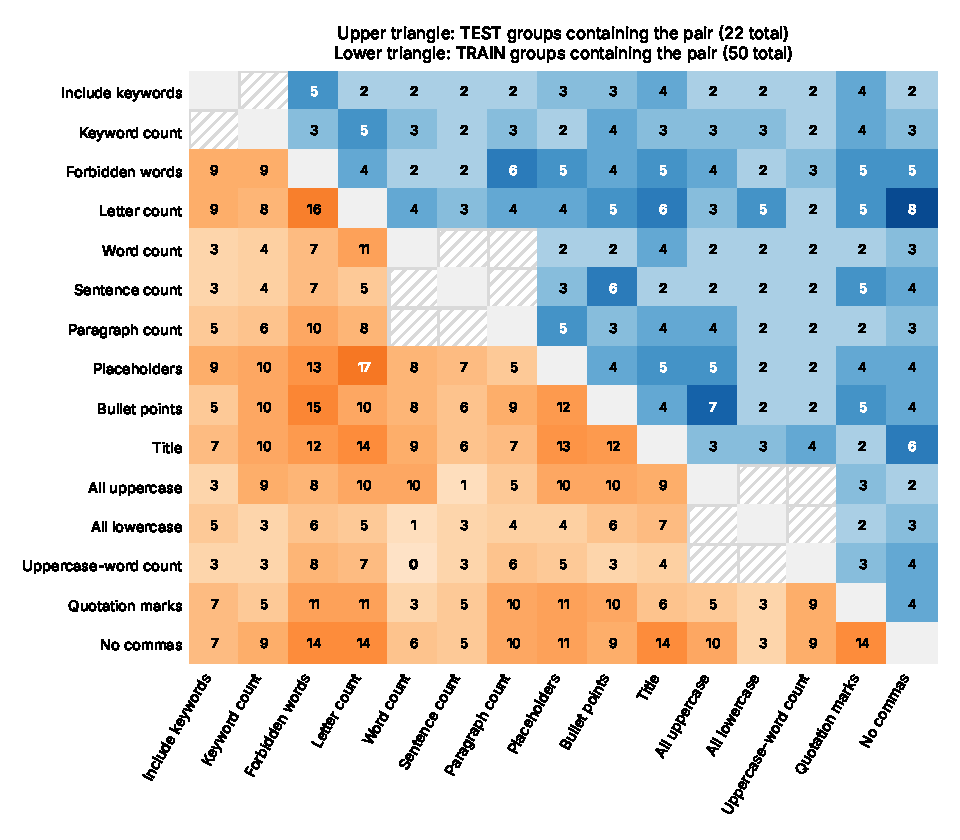
\includegraphics[width=0.8\linewidth]{figures/pair_coverage_s3.pdf}
\caption{Pair coverage of the adopted split: the number of test groups (upper triangle) and training groups (lower
triangle) whose rule pool contains both types. Hatched cells are type pairs that ManyIFEval never combines. Derived
from pool metadata only.}
\label{fig:pairs}
\end{figure}

\section{Feature and fitting details}
\label{app:recipe}

\textbf{Hidden-state rows.} Row 0 holds token embeddings, rows $1,\dots,L-1$ the outputs of decoder layers
$1,\dots,L-1$, row $L$ the last layer after the final normalisation and row $L+1$ the last layer before it ($L=32$ for
Llama, 36 for Qwen). The candidate rows are 8, 12, 16, 24 and 33 for Llama and 9, 14, 18, 27 and 37 for Qwen, so the
deepest candidate is the un-normalised residual stream of the last layer.

\textbf{Attention extraction.} The eager kernel returns bfloat16 probabilities, so each maximum is itself a bfloat16
value and is stored losslessly. Before the full pass we checked, on fixed training prompts including multi-token rules
and spans whose boundary token straddles whitespace, that each indexed span covers exactly the rule's tokens and that
the extracted value equals the direct maximum from the full attention row for every layer and head.

\textbf{Solver.} Each head is fitted by damped Newton iterations with the exact Hessian (float64 gradient and Cholesky
factorisation), warm-started along the penalty path from strong to weak, and stopped when the largest gradient entry
falls below $10^{-9}$ on the mean scale. Exact-rule embedding blocks are replaced, per head and fold, by coordinates in
an orthonormal basis of their row space on the fitting rows, which is exact for ridge and much faster because a head
sees few distinct rules.

\textbf{Objective~2 structure.} $k$, rendered prompt length, and for each of five ordered slots the one-hot rule type
(15), span length, distance from the span end to the final token and a presence mask: $2+5\times18=92$ columns.

\section{Training cross-validation diagnostics}
\label{app:cv}

Table~\ref{tab:cv} lists the pooled cross-validation loss of each predictor at its selected setting. These are the
criteria used for selection, computed on the 50 training groups only; they are optimistically biased, carry no
uncertainty estimate and are \emph{not} estimates of held-out performance. They are reported to document the selection,
not to support any comparison.

\begin{table}[h]
\centering\footnotesize
\caption{Training cross-validation loss at the selected setting (5 grouped folds over the 50 training groups) and the
number of input features. Objective~1: pooled mean log loss per completion. Objective~2: pooled squared error of
$\hat q$, $\times10^3$. Generated from \texttt{results/v2\_s3/tables/selected\_settings.csv}.}
\label{tab:cv}
\setlength{\tabcolsep}{2.8pt}
% generated by report/neurips_draft/make_assets.py from results/v2_s3/tables/selected_settings.csv
\begin{tabular}{lrrrrrrrr}
\toprule
 & \multicolumn{4}{c}{Obj.~1: log loss} & \multicolumn{4}{c}{Obj.~2: MSE ($\times 10^{3}$)} \\
\cmidrule(lr){2-5}\cmidrule(lr){6-9}
Predictor & \multicolumn{2}{c}{Llama} & \multicolumn{2}{c}{Qwen} & \multicolumn{2}{c}{Llama} & \multicolumn{2}{c}{Qwen} \\
 & loss & dim. & loss & dim. & MSE & dim. & MSE & dim. \\
\midrule
Structure only (S) & 0.5035 & 20 & 0.3560 & 20 & 21.830 & 92 & 14.020 & 92 \\
\midrule
B1 (S\,+\,P) & 0.4820 & 1044 & 0.3404 & 1044 & 21.365 & 1116 & 13.931 & 1116 \\
B2 (S\,+\,P\,+\,R) & 0.4013 & 2068 & 0.2927 & 2068 & 17.607 & 2140 & 13.224 & 2140 \\
H1\,+\,S & 0.4138 & 4116 & 0.2822 & 4116 & 16.059 & 4188 & 12.192 & 4188 \\
H2\,+\,S & 0.3934 & 5140 & 0.2741 & 5140 & 16.051 & 5212 & 12.122 & 5212 \\
RCAP (A\,+\,R\,+\,S) & 0.3897 & 2068 & 0.2741 & 2196 & 15.657 & 2140 & 12.105 & 2268 \\
\midrule
B1\,+\,H1 & 0.4131 & 5140 & 0.2880 & 5140 & 16.115 & 5212 & 12.225 & 5212 \\
B2\,+\,H1 & 0.3849 & 6164 & 0.2741 & 6164 & 16.203 & 6236 & 12.187 & 6236 \\
B2\,+\,A1 & 0.3821 & 3092 & 0.2734 & 3220 & 15.674 & 3164 & 12.514 & 3292 \\
Other generator's H1\,+\,S & 0.3974 & 4116 & 0.2894 & 4116 & 16.815 & 4188 & 11.608 & 4188 \\
\bottomrule
\end{tabular}

\end{table}

\section{Project history and pre-registration log}
\label{app:history}

An earlier version of the analysis compared 23 feature configurations per objective, stacked on two baselines, with MLP
and linear heads and a fine-tuned (LoRA) text encoder. A design review on training data found that adding a probe to a
baseline did not isolate the probe: in Objective~1 the baselines used one shared head while every configuration with a
probe used per-type heads, many configurations had identical inputs, one shared penalty over concatenated blocks made
fusions non-nested, and there was no cross-generator control. The current analysis (Section~\ref{sec:methods}) was
adopted in response, before any test row was read, with the fitting recipe hashed before selection. The test split was
then enlarged from 15 to 22 groups to guarantee pair coverage, the training-only features were rebuilt, and selection
and refitting were rerun under the new split. The earlier plan, its frozen analysis file and all earlier results are
preserved unchanged.

\section{Compute}
\label{app:compute}

Generation ran with vLLM 0.25.0 in bfloat16 on single NVIDIA B200 GPUs; in the 2,000-response pilot, throughput was
about 24,000 output tokens per second for Llama and 19,000 for Qwen. Pre-generation features were extracted on an Apple
M4 Max laptop (64\,GB unified memory) with PyTorch MPS. The maximum-attention store takes about 0.5\,GB per generator.
All probe fitting ran on the same laptop.

\section{Reproducibility and use of AI tools}
\label{app:repro}

\paragraph{Reproducibility.} The ManyIFEval commit, model revisions, chat templates, decoding settings, seeds and
package versions are pinned and recorded. Generation, verification and feature extraction are resumable and write
hashed manifests, and every artifact of the analysis carries a version key that loaders check. The fitting recipe was
hashed before selection, and every number in this report is generated from saved tables by a script. We will release
the manifest, labels, features and code.

\paragraph{Use of AI tools.} An AI coding assistant was used, under the authors' direction, to implement the pipeline,
run analyses and draft text. The authors reviewed the work and are responsible for its content.


\end{document}
